\documentclass[twocolumn]{article}

% affiliation
\usepackage[affil-it]{authblk}
% Language setting
% Replace `english' with e.g. `spanish' to change the document language
\usepackage[english]{babel}

% For subfigure use
\usepackage[font=small,labelfont=bf]{caption}
\usepackage{subcaption}

% change title font
\usepackage{sectsty}
\sectionfont{\fontsize{12}{12}\selectfont}
\subsectionfont{\fontsize{11}{11}\selectfont}

% Set page size and margins
% Replace `letterpaper' with`a4paper' for UK/EU standard size
\usepackage[a4paper,top=2cm,bottom=2cm,left=1.5cm,right=1.5cm,marginparwidth=1.6cm]{geometry}
\raggedbottom

% tabelas
\usepackage{array}
\usepackage{tabularx}
\usepackage{multirow}
\usepackage{booktabs}
\usepackage[table,xcdraw]{xcolor}

\usepackage{float}

% Useful packages
\usepackage{amsmath}
\usepackage{graphicx}
\graphicspath{{figures/}} %Setting the graphicspath
\usepackage[colorlinks=true, allcolors=blue]{hyperref}

\title{Neural Networks applied to Structure Health Monitoring using autoregressive models as feature extractors}
\author{Felipe da Costa Pereira - (felipecostapereira@gmail.com)}
\affil{PUC-RJ - ELE2389 - Redes Neurais - Trabalho Final}
\affil{Professora: Marley Vellasco}

\begin{document}
\maketitle

%      _    ____ ____ _____ ____      _    ____ _____
%     / \  | __ ) ___|_   _|  _ \    / \  / ___|_   _|
%    / _ \ |  _ \___ \ | | | |_) |  / _ \| |     | |
%   / ___ \| |_) |__) || | |  _ <  / ___ \ |___  | |
%  /_/   \_\____/____/ |_| |_| \_\/_/   \_\____| |_|

\begin{abstract}

In Structure Health Monitoring, an important task is to detect damage patterns in a given physical system. Machine Learning techniques have been successfully applied in this area for this purpose. A critical step in a machine learning project is the feature extraction, as measured data acquired in these systems usually consist of important amount of timeseries information. This paper proposes a complete data processing pipeline, from feature extraction based on autoregressive models to state condition damage detection classification, using neural networks and comparing its preformance with other popular classification algorithms and based on a laboratory data acquisition assembly. This work also analyses a neural network based Kohonen Map as an unsupervised method to understand the feature space for the problem of damage detection in SHM.



\end{abstract}

%   ___ _   _ _____ ____   ___  ____  _   _  ____    _    ___
%  |_ _| \ | |_   _|  _ \ / _ \|  _ \| | | |/ ___|  / \  / _ \
%   | ||  \| | | | | |_) | | | | | | | | | | |     / _ \| | | |
%   | || |\  | | | |  _ <| |_| | |_| | |_| | |___ / ___ \ |_| |
%  |___|_| \_| |_| |_| \_\\___/|____/ \___/ \____/_/   \_\___/


\section{Introduction}

Structure Health Monitoring (SHM) consists of observing measured data from a given physical system in order to monitor properties and characteristics over time. Damage detection is one of the important objectives of this discipline, as it tries to detect, in advance, a failure event that can occur when the system is operating ou of its normal condition.

The measured data in this field consists of sensors response over time. The main approach to detect damage is try to select features from these data that are sensitive to damage but insensitive to operational and environmental variations (\cite{autoreg}). In \cite{report_dataset}, a complete discussion on several techniques for feature extraction can be found and the paradigms of feature extraction for strucutre health monitoring are widely discussed in \cite{axioms}.

Autoregressive models are a class of models which can be succesfully applied for feature extraction. The work \cite{autoreg} analyses in detail the autoregressive (AR) timeseries models as feature extractor tools in order to detect damage patterns on a laboratory experiment. Such study also shows the importance of the model order as a key parameter to represent the patterns. According to the autors, the AR model coefficients are, themselves, sensitive features to the damage, since the appropriate model order is respected.

The approach of this case study is to use neural networks to identify damage in a controlled experiment, using the autoregressive (AR) models as feature exractors as disucssed in \cite{autoreg}, and its coefficients as features. Then, we compare the results with other popular algorithms for classification.

%   _______  ______  _____ ____  ___ __  __ _____ _   _ _____  _    _
%  | ____\ \/ /  _ \| ____|  _ \|_ _|  \/  | ____| \ | |_   _|/ \  | |
%  |  _|  \  /| |_) |  _| | |_) || || |\/| |  _| |  \| | | | / _ \ | |
%  | |___ /  \|  __/| |___|  _ < | || |  | | |___| |\  | | |/ ___ \| |___
%  |_____/_/\_\_|___|_____|_| \_\___|_|  |_|_____|_| \_| |_/_/   \_\_____|
%  |  _ \  / \|_   _|/ \
%  | | | |/ _ \ | | / _ \
%  | |_| / ___ \| |/ ___ \
%  |____/_/   \_\_/_/   \_\

\section{Experimental Data}

Several studies in SHM are conducted using standard datasets. In this study we will use a dataset consisting of measures from a three-floor structure assembled in the Los Alamos National Laboratory (LANL). The structure has different columns and plates connected by joints. Different damage scenarios are simulated by adjusting the gap between column and bumper in the middle of the top floor (figure \ref{fig:experiment02}). Environmental conditions are simulated varying the stiffness of some columns (figure \ref{fig:experiment01}) and adding mass to some plates (figure \ref{fig:experiment02}).

\begin{figure}[H]
      \centering
      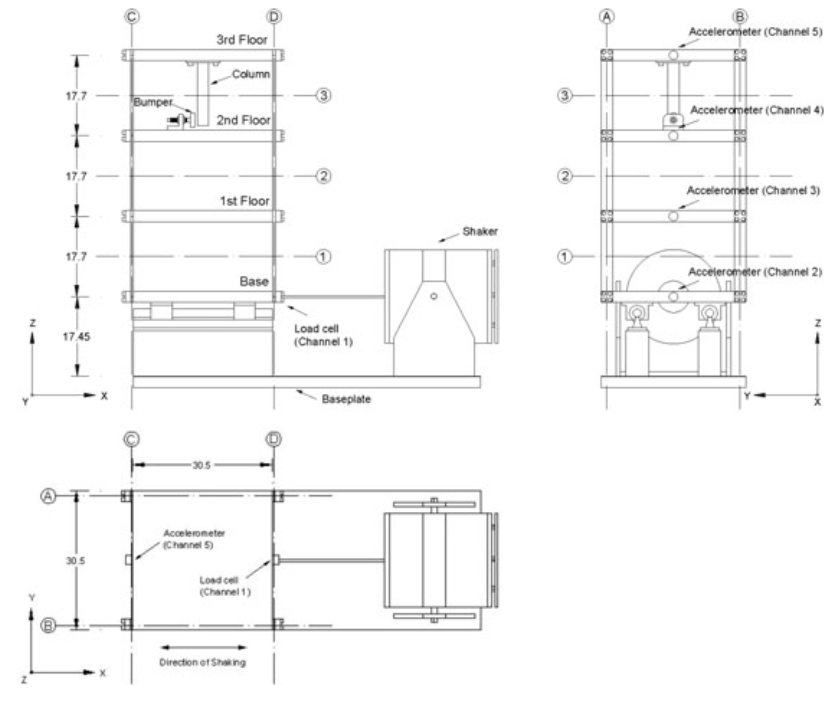
\includegraphics[width=0.45\textwidth]{experiment_01.PNG}
      \caption{General overview of the three stage model}
      \label{fig:experiment01}
\end{figure}

\begin{figure}[H]
      \centering
      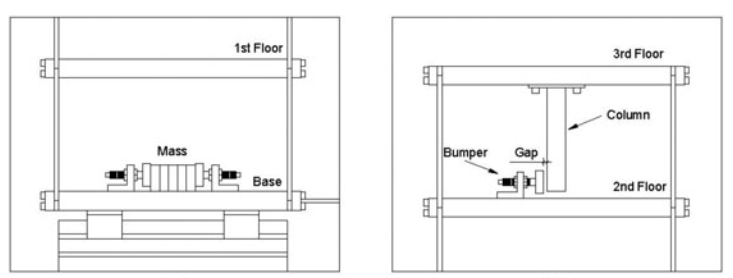
\includegraphics[width=0.3\textwidth]{experiment_02.PNG}
      \caption{Sources of environmental and non-linear effects}
      \label{fig:experiment02}
\end{figure}

The model is composed of four sensors (accelerometers) that register the vibration measures from the base and the three floors as seen in figure \ref{fig:experiment01}. For a given case, each channel accelerometer captures a set of 8192 datapoins correspondig to a time window of about 26 seconds. The details of the given structure and the data used in our case-study are described in \cite{report_dataset}.

A total of 50 measures were made for each one of the 17 state conditions described in table \ref{table:statesTable}, what gives a total of 850 observations in the dataset. The state conditions can be grouped as shown in table \ref{table:GroupTable} according to the kind of stimulation imposed to the structure.

\begin{table}[H]
      \small
      \centering
      \caption{Labels for the 17 state conditions}
      \begin{tabular}{ m{1.4em} m{1.6cm} m{5cm}}
            State &  Condition & Description \\
            \hline
            \#1 & Undamaged & Baseline condition \\
            % \hline
            \#2 & Undamaged & Mass=1.2kg(base) \\
            \#3 & Undamaged & Mass=1.2kg(1st floor) \\
            \#4 & Undamaged & 87.5\% stiffness drop (1BD) \\
            \#5 & Undamaged & 87.5\% stiffness drop (1AD-1BD) \\
            \#6 & Undamaged & 87.5\% stiffness drop (2BD) \\
            \#7 & Undamaged & 87.5\% stiffness drop (2AD-2BD)\\
            \#8 & Undamaged & 87.5\% stiffness drop (3BD) \\
            \#9 & Undamaged & 87.5\% stiffness drop (3AD-3BD) \\
            % \hline
            \#10 & Damaged & Gap=0.20mm \\
            \#11 & Damaged & Gap=0.15mm \\
            \#12 & Damaged & Gap=0.13mm \\
            \#13 & Damaged & Gap=0.10mm \\
            \#14 & Damaged & Gap=0.05mm \\
            % \hline
            \#15 & Damaged & Gap=0.20mm, mass=1.2kg (base) \\
            \#16 & Damaged & Gap=0.20mm, m=1.2kg (1st floor) \\
            \#17 & Damaged & Gap=0.10mm, m=1.2kg (1st floor)
      \end{tabular}
      \label{table:statesTable}
\end{table}

\begin{table}[H]
      \small
      \centering
      \caption{Grouped classes}
      \begin{tabular}{ccc}
            State &  Group & Description \\
            \hline
            1 & 1 & Baseline Condition \\
            2,3,4,5,6,7,8,9 & 2 & Environmental Change only \\
            10,11,12,13,14  & 3 & Damage only \\
            15,16,17 & 4 & Damaged/Environmental Change
      \end{tabular}
      \label{table:GroupTable}
\end{table}

Each case (observation) consists of the measures of 4 accelerometers composed by 8192 datapoints each. By concatenating the information from the four channels, the dataset is composed by 850 rows (cases) and (4 x 8192 = 32768) datapoints, which are considered as features. The timeseries for two of these observations (cases) are show in figure \ref{fig:cases_000_790}, where force and accelerations form the four measure channels are plotted. The plots in the right shows a detail of the first 60 datapoints either for the force and for the 4 accelerometers.

\begin{figure}[H]
      \centering
      \begin{subfigure}{0.4\textwidth}
            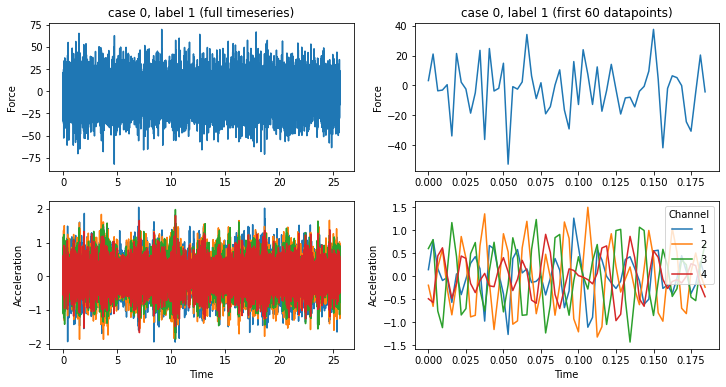
\includegraphics[width=\textwidth]{case_000.png}
            \caption{Case (observation) \#0, State Condition (class) \#1}
            \label{fig:case_000}
      \end{subfigure}
      \begin{subfigure}{0.4\textwidth}
            \centering
            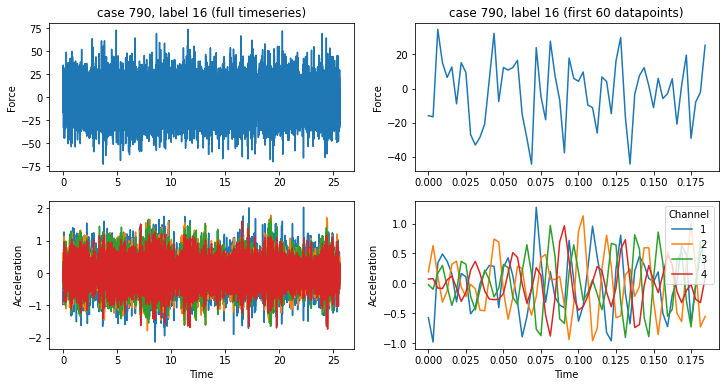
\includegraphics[width=\textwidth]{case_790.png}
            \caption{Case (observation) \#790, State Condition (class) \#16}
            \label{fig:case_790}
      \end{subfigure}
      \caption{Measured timeseries for two of the 850 cases}
      \label{fig:cases_000_790}
\end{figure}


%   __  __ _____ _____ _   _  ___  ____   ___  _     ___   ______   __
%  |  \/  | ____|_   _| | | |/ _ \|  _ \ / _ \| |   / _ \ / ___\ \ / /
%  | |\/| |  _|   | | | |_| | | | | | | | | | | |  | | | | |  _ \ V /
%  | |  | | |___  | | |  _  | |_| | |_| | |_| | |__| |_| | |_| | | |
%  |_|  |_|_____| |_| |_| |_|\___/|____/ \___/|_____\___/ \____| |_|

\section{Methodology}

The Data Procesing Pipeline used in this study is shown in figure \ref{fig:dip}. The first step is to apply the autoregressive model to the measured data. As a high number of features is kept after applying the AR model, we use then a PCA to reduce the dataset dimensionallity. As a third step we make an exploratory analysis in order to get insights about the dataset and the classes distributions, followed by a data preparation step. The two final steps, model training and evaluation will be detailed in the next sessions, as we define the model validation protocol.

\begin{figure*}[h!]
      \centering
      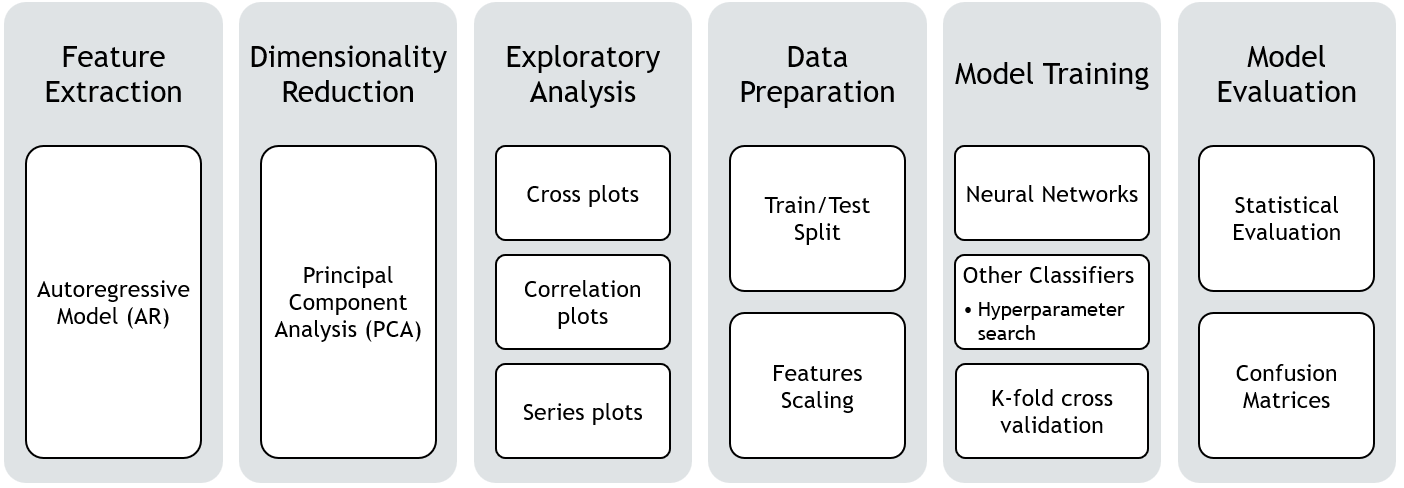
\includegraphics[width=0.75\textwidth]{DIP.PNG}
      \caption{Data Procesing Pipeline}
      \label{fig:dip}
\end{figure*}

%   _____ _____    _  _____   _______  _______ ____      _    ____ _____ ___ ___  _   _
%  |  ___| ____|  / \|_   _| | ____\ \/ /_   _|  _ \    / \  / ___|_   _|_ _/ _ \| \ | |
%  | |_  |  _|   / _ \ | |   |  _|  \  /  | | | |_) |  / _ \| |     | |  | | | | |  \| |
%  |  _| | |___ / ___ \| |   | |___ /  \  | | |  _ <  / ___ \ |___  | |  | | |_| | |\  |
%  |_|   |_____/_/   \_\_|   |_____/_/\_\ |_| |_| \_\/_/   \_\____| |_| |___\___/|_| \_|


\section{Feature Extraction - Auto Regressive Models}

The AR($p$) model, where $p$ defines the order or number of parameters in the model, is developed from
response time-series data $x_1, x_2, \cdots, x_n$ and it can be written as

\[x_i = \sum_{j=1}^{p} \phi_j x_{i-j} + \epsilon_i\]

where $xi$ is the measured signal at the time instant $ti$. The parameters $\phi_j$ are fitted so that the residual in predicting the value of the timeseries $x_i$ , using the previous values $x_{i-j}$, is minimized. This estimation of the unknown AR parameters, $\phi_j$, can be done by using least-squares approach and the $\phi_j$ parameters can be used directly as damage-sensitive features. The appropriate AR model order is initially unknown. A higher order model may better fit the data, but may not generalize well to other data sets. On the other hand, a low-order model will not necessarily capture the underlying physical system dynamics \cite{autoreg}.

In this study we will use $p = 30$ as proposed by \cite{autoreg} as being a good model order to work as a feature extractor for the database used. By fitting the AR(p=30) model for each one of the four channels we have 30 coefficients per channel. We apply the AR(30) model to each of the four channels timeseries of all the 850 cases in the dataset. Each channel 8192 datapoints are then transformed into the domain of the 30 AR coefficients. The mean value of the AR model parameters, computed in the 850 dataset observations is shown in figure \ref{fig:ar0}, for the four accelerometers measures.

\begin{figure}[H]
      \centering
      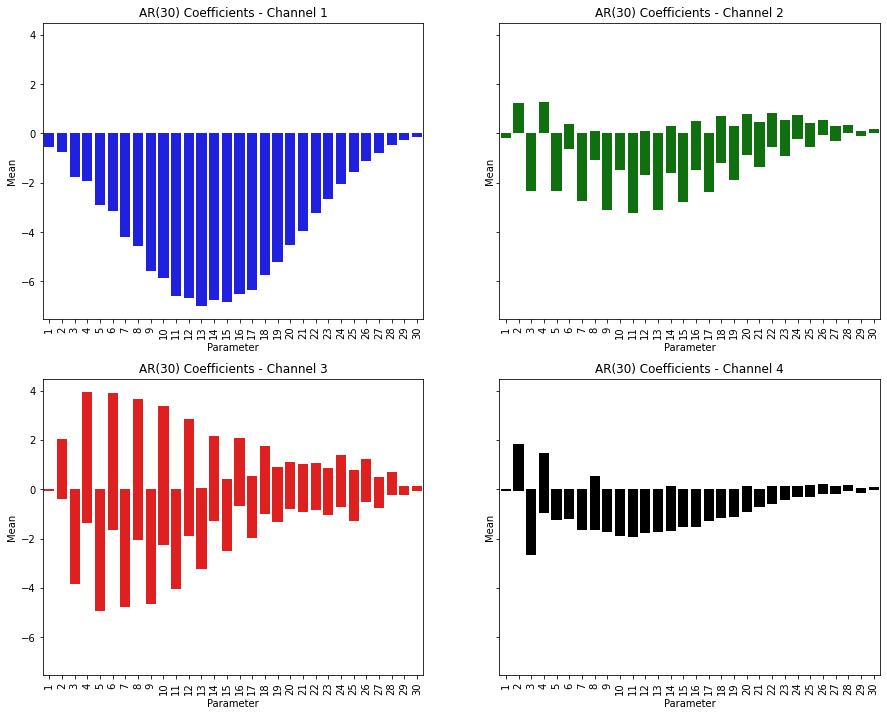
\includegraphics[width=0.5\textwidth]{ar_0.png}
      \caption{Mean value of the AR(30) coeffients, for each one of the four channels, computed over the 850 cases}
      \label{fig:ar0}
\end{figure}

To represent the complete set of measured data as being the complete set the 4 channels information, we then concatenate the 30 parameters for the four channels, wich gives a total of 120 features for each of the 850 cases in the dataset. Figure \ref{fig:ar1} shows a plot of the 120 composed feature set of the 850 measured cases.

\begin{figure}[H]
      \centering
      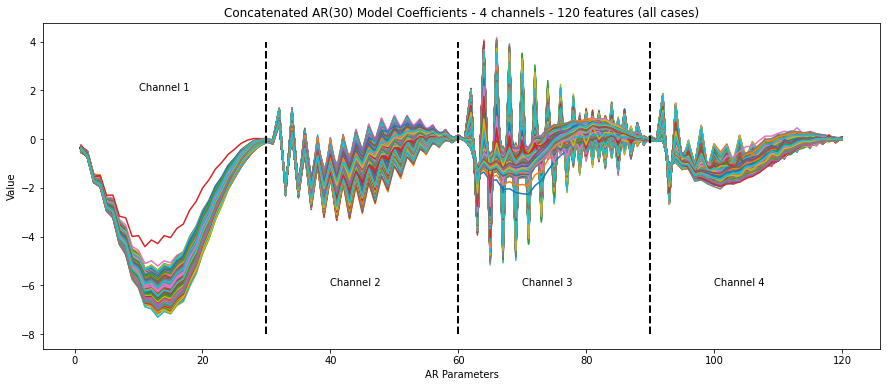
\includegraphics[width=0.5\textwidth]{ar_1.png}
      \caption{850 cases x 120 feautures (AR Model parameters), 4 channels concatenated}
      \label{fig:ar1}
\end{figure}

At this point, the total number of features is still high to be used directly as a feature input space for any classification model, as it can lead to overfitting issues. In figure \ref{fig:ar2} we can see a correlation matrix between these 120 features. As high correlations are shown between some features,specially when it comes to channel 1 and 2 (first 60 parameters), we need to reduce the dimensionallity of this input space. To address this issue, we will apply a PCA analysis.

\begin{figure}[H]
      \centering
      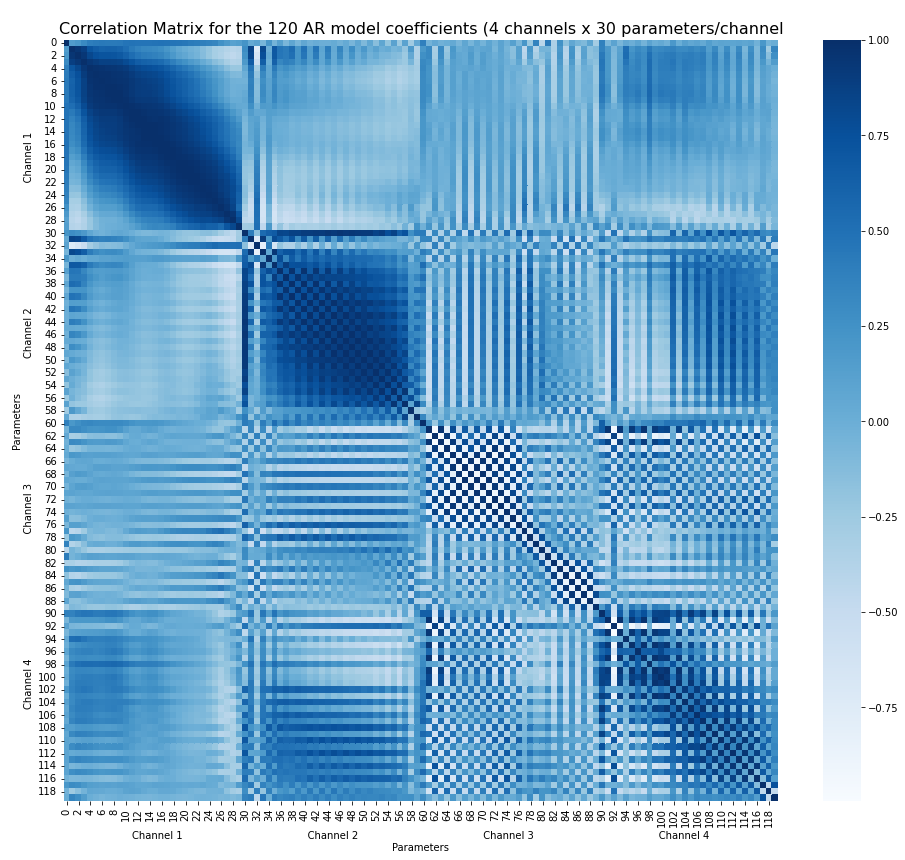
\includegraphics[width=0.5\textwidth]{ar_2.png}
      \caption{Correlation matrix between the features given by the AR Model}
      \label{fig:ar2}
\end{figure}

%   ____ ___ __  __   ____  _____ ____  _   _  ____ _____ ___ ___  _   _
%  |  _ \_ _|  \/  | |  _ \| ____|  _ \| | | |/ ___|_   _|_ _/ _ \| \ | |
%  | | | | || |\/| | | |_) |  _| | | | | | | | |     | |  | | | | |  \| |
%  | |_| | || |  | | |  _ <| |___| |_| | |_| | |___  | |  | | |_| | |\  |
%  |____/___|_|  |_| |_| \_\_____|____/ \___/ \____| |_| |___\___/|_| \_|

\section{Dimensionality Reduction - PCA}

Large or massive data sets are increasingly common and often include measurements on many variables. It is frequently possible to reduce the number of variables considerably while still retaining much of the information in the original data set. Principal component analysis (PCA) is probably the best known and most widely used dimension-reducing technique for doing this. PCA finds linear combinations of the original variables, called principal components, that successively have maximum variance for the data \cite{pca}.

In this study we apply a PCA transformation on the features provided by the AR Model. Figure \ref{fig:pca0} shows a relation between the number of PCA components and the explained variance of the data. For the next steps we choose to use the 6 first PCA components, which are responsable to represent 96\% of the variance.

\begin{figure}[H]
      \centering
      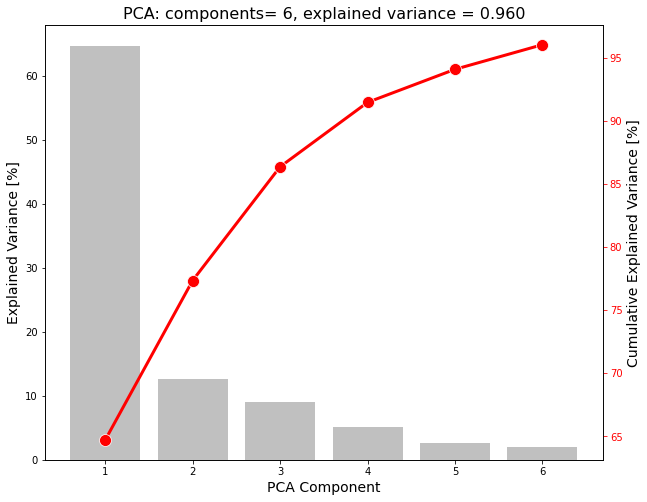
\includegraphics[width=0.5\textwidth]{pca_0.png}
      \caption{PCA explained variance sensibility to the number of components chosen}
      \label{fig:pca0}
\end{figure}

%
%   _______  ______  _     ___  ____      _  _____ ___  ______   __     _    _   _    _    _  __   ______ ___ ____
%  | ____\ \/ /  _ \| |   / _ \|  _ \    / \|_   _/ _ \|  _ \ \ / /    / \  | \ | |  / \  | | \ \ / / ___|_ _/ ___|
%  |  _|  \  /| |_) | |  | | | | |_) |  / _ \ | || | | | |_) \ V /    / _ \ |  \| | / _ \ | |  \ V /\___ \| |\___ \
%  | |___ /  \|  __/| |__| |_| |  _ <  / ___ \| || |_| |  _ < | |    / ___ \| |\  |/ ___ \| |___| |  ___) | | ___) |
%  |_____/_/\_\_|   |_____\___/|_| \_\/_/   \_\_| \___/|_| \_\|_|   /_/   \_\_| \_/_/   \_\_____|_| |____/___|____/
%
\section{Exploratory Analysis}

After transforming the data with the Principal Component technique, the feature space drops to six representative features. As shown in \ref*{fig:exploratory_01}, the first PCA component carries information to distinguish some of the 17 state conditions. PCA components 2 and 3 also carry information to detect some labels but have more similar values between the classes. For the fourth PCA component, the 17 classes have similar values.

\begin{figure}[H]
      \centering
      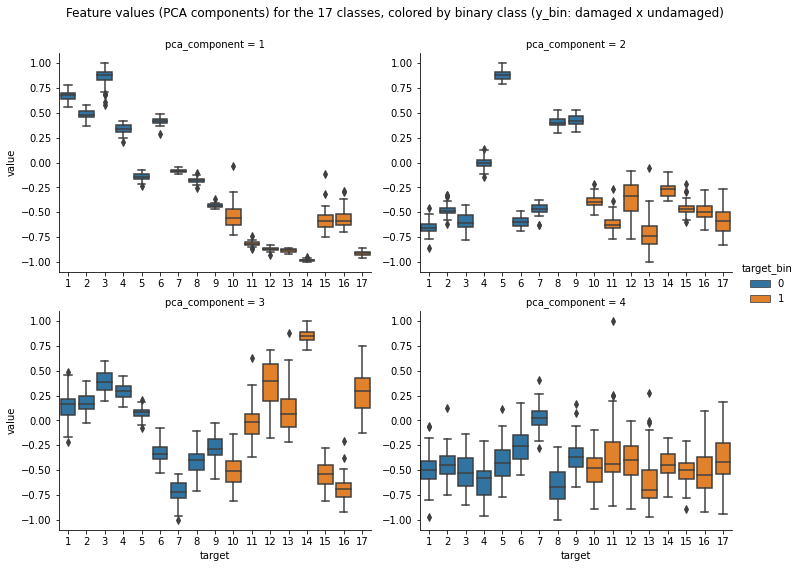
\includegraphics[width=0.5\textwidth]{exploratory_01.png}
      \caption{Distribution of the first four PCA component values for each one of the 17 state conditions}
      \label{fig:exploratory_01}
\end{figure}

The cross plots in figure \ref*{fig:pairplots} show a relationship between components 1 and the other to most imporatant (2 and three). In the binary class problem (figure \ref*{fig:pairplot_bin}), the classes seem to be linearly separable. On the other hand, for the 4 group and 17 state conditions classification, the classes are mixed in the space of features given by PCA components.

\begin{figure}[H]
      \centering
      \begin{subfigure}{0.4\textwidth}
            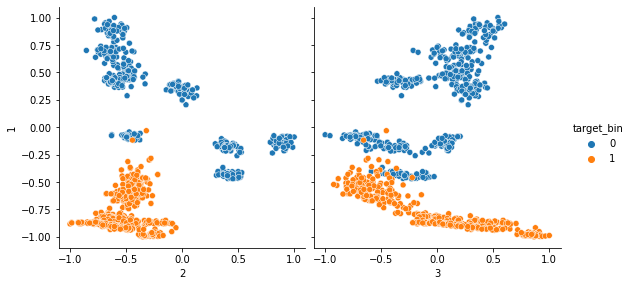
\includegraphics[width=\textwidth]{pairplot_bin.png}
            \caption{binary classification}
            \label{fig:pairplot_bin}
      \end{subfigure}
      \begin{subfigure}{0.4\textwidth}
            \centering
            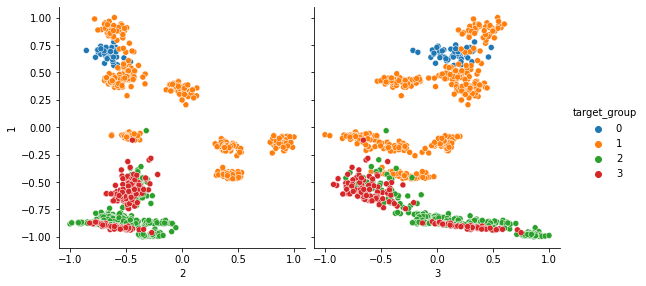
\includegraphics[width=\textwidth]{pairplot_04.png}
            \caption{four groups classification}
            \label{fig:pairplot_04}
      \end{subfigure}
      \begin{subfigure}{0.4\textwidth}
            \centering
            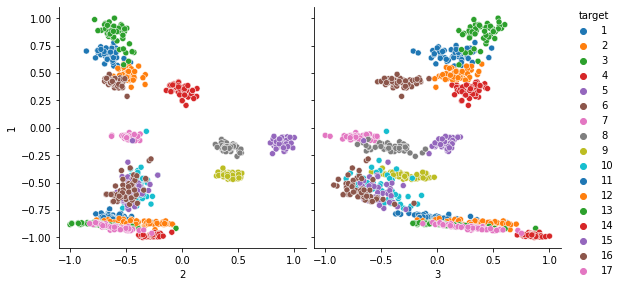
\includegraphics[width=\textwidth]{pairplot_17.png}
            \caption{17 state conditions}
            \label{fig:pairplot_17}
      \end{subfigure}
      \caption{Crossplots between PCA components 1,2 and three for the three levels of classification}
      \label{fig:pairplots}
\end{figure}

%    ____ _        _    ____ ____ ___ _____ ___ ____    _  _____ ___ ___  _   _
%   / ___| |      / \  / ___/ ___|_ _|  ___|_ _/ ___|  / \|_   _|_ _/ _ \| \ | |
%  | |   | |     / _ \ \___ \___ \| || |_   | | |     / _ \ | |  | | | | |  \| |
%  | |___| |___ / ___ \ ___) |__) | ||  _|  | | |___ / ___ \| |  | | |_| | |\  |
%   \____|_____/_/   \_\____/____/___|_|   |___\____/_/   \_\_| |___\___/|_| \_|

\section{Classification}

%      _    _   _ _   _
%     / \  | \ | | \ | |
%    / _ \ |  \| |  \| |
%   / ___ \| |\  | |\  |
%  /_/   \_\_| \_|_| \_|


\subsection{Neural Networks}

A neural network is a machine that is designed to model the way in which the brain performs a particular task or function of interest: the network is usually implemented by using electronic components or is simulated in software on a digital computer. To achieve good performance, neural networks employ a massive interconnection of simple computing cells referred to as "neurons" or "processing units". A neural network is a massively parallel distributed processor made up of simple processing units that has a natural propensity for storing experiential knowledge and making it available for use. The procedure used to perform the learning process is called a learning algorithm, the function of which is to modify the synaptic weights to attain a desired design objective. The modification of synaptic weights provides the traditional method for the design of neural networks \cite{haykin2}

In this study, we'll train a Multi Layer Perceptron (MLP) neural network to predict the damage classes in the three store dataset using the backpropagtion method \cite{haykin2}. In order to prevent the model from overfitting, we avoid to choose a very large number of neurons acording to the metric proposed in \cite{HECHTNIELSEN199265}:

\[N_{hidden} <= 2N_{input} + 1\]

Other parameters were tested: number of hidden layers (one or two), learning rate, number of epochs, type of acivation function for the hidden processors. The neural network clasifier architecture (one relu activation hidden layer with 13 processors) was chosen over a 5-fold cross-validation as the model having the best score over the five folds.


As a second step, we used the selected model to measure its behaviour on different holdout sets by training that model once again for each of the ten train/validation/test splits as described in figure \ref{fig:ann_protocol}. The objective of this step is to provide a statistical assessment of the results by eliminating possible biases if a single holdout was used.

\begin{figure}[H]
      \centering
      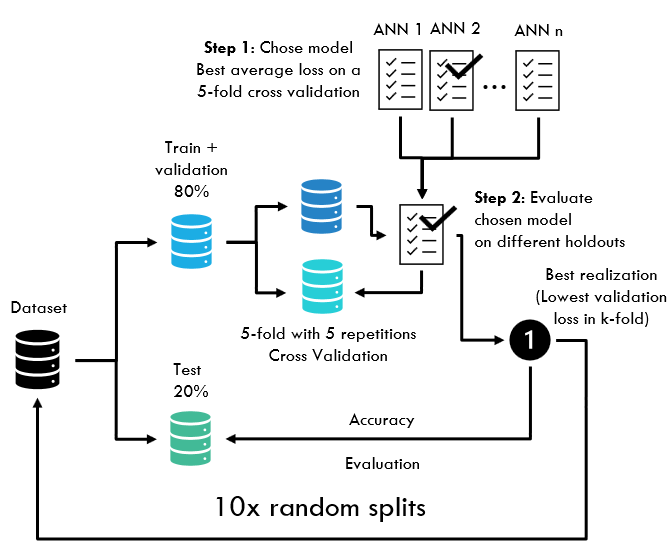
\includegraphics[width=0.5\textwidth]{ann_protocol.png}
      \caption{Neural network model selection and performance measure scheme}
      \label{fig:ann_protocol}
\end{figure}


The selected architecture was: 6 input (PCA components), 13 hidden neurons in 1 hidden layer, softmax activation function for the output and relu for the hidden layer. Concerning the output, this architecture was tested in two situations: predicting the 17 damage states and predicting the 4 group (\ref{table:GroupTable}). The procedure described in \ref*{fig:ann_protocol} was executed then, twice, with 17 and 4 outputs, respectivelly.

The confusion matrices (normalized by the true label), for these two problems, is shown in \ref{fig:confusion_matrix}, for the best realization model over the 10 different splits. Although the model had a higher accuracy on predicting the four grouped stage conditions compared to the 17 classes, the results were quite similar in terms of accuracy.

\begin{figure*}[t!]
      \centering
      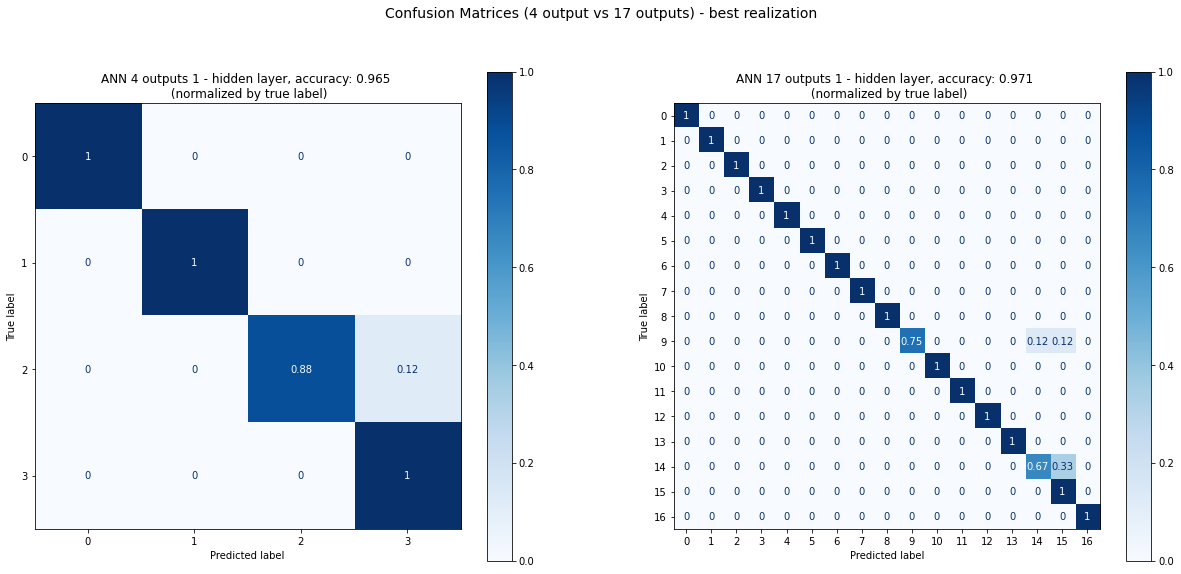
\includegraphics[width=0.9\textwidth]{confusion_matrix.png}
      \caption{Neural network performance on predicting 4 groups (accuracy=0.971) or 17 classes (accuracy=0.953)}
      \label{fig:confusion_matrix}
\end{figure*}

%    ___ _____ _   _ _____ ____     ____ _        _    ____ ____ ___ _____ ___ _____ ____  ____
%   / _ \_   _| | | | ____|  _ \   / ___| |      / \  / ___/ ___|_ _|  ___|_ _| ____|  _ \/ ___|
%  | | | || | | |_| |  _| | |_) | | |   | |     / _ \ \___ \___ \| || |_   | ||  _| | |_) \___ \
%  | |_| || | |  _  | |___|  _ <  | |___| |___ / ___ \ ___) |__) | ||  _|  | || |___|  _ < ___) |
%   \___/ |_| |_| |_|_____|_| \_\  \____|_____/_/   \_\____/____/___|_|   |___|_____|_| \_\____/

\subsection{Other Classifiers}

As the neural network trained in the previous section could work as a good predictor either for the 17 state conditions or the 4 grouped states, another objecitve of this study is to compare its performance with other known classifiers. The most popular algortihms in machine learning were included for that purpose.

Since the neural network parameters (weights) learn through time with the backpropagation algorithm of trainning, we also provide a hyperparameter search for the soft classifiers, in order to tune them to get a more reliable comparison. A list of classifiers and the respecitve parameters used in hyperparameter search is found in table \ref*{tab:soft_parameters}.

\begin{table}[H]
      \centering
      % \small
      \caption{Soft classifiers parameters used in hyperparameter search}
      \resizebox{\columnwidth}{!}{%
      \begin{tabular}{@{}ccc@{}}
            \toprule
            Classifier                      & Parameter      & Value Range                        \\ \midrule
            Gaussian Naive-Bayes            & -              & -                                  \\
            \rowcolor[HTML]{EFEFEF}
            \cellcolor[HTML]{EFEFEF}        & penalty       & 'l1', 'l2', 'elasticnet', 'none'          \\
            \rowcolor[HTML]{EFEFEF}
            \cellcolor[HTML]{EFEFEF}        & C              & 1-25                               \\
            \rowcolor[HTML]{EFEFEF}
            \multirow{-3}{*}{\cellcolor[HTML]{EFEFEF}Logistic Regression}  & solver        & 'newton-cg', 'sag', 'saga', 'lbfgs'       \\
                                          & C              & 1-25                               \\
                                          & kernel         & 'linear', 'poly', 'rbf', 'sigmoid' \\
                                          \multirow{-3}{*}{SVM}           & degree         & 1-10                               \\
                                          \rowcolor[HTML]{EFEFEF}
            \cellcolor[HTML]{EFEFEF}        & n\_neighbors   & 3-11                               \\
            \rowcolor[HTML]{EFEFEF}
            \cellcolor[HTML]{EFEFEF}                                     & algorithm     & 'auto', 'ball\_tree', 'kd\_tree', 'brute' \\
            \rowcolor[HTML]{EFEFEF}
            \multirow{-3}{*}{\cellcolor[HTML]{EFEFEF}K-nearest neighbors}                & leaf\_size    & 1-50                                      \\
            & criterion      & 'gini', 'entropy'                  \\
                                          & max\_features  & 0-1                                \\
                                          \multirow{-3}{*}{Decision Tree} & max\_depth     & 3-20                               \\
            \rowcolor[HTML]{EFEFEF}
            \cellcolor[HTML]{EFEFEF}        & n\_estimators  & 2-100                              \\
            \rowcolor[HTML]{EFEFEF}
            \cellcolor[HTML]{EFEFEF}        & criterion      & 'gini', 'entropy'                  \\
            \rowcolor[HTML]{EFEFEF}
            \cellcolor[HTML]{EFEFEF}        & max\_features  & 0-1                                \\
            \rowcolor[HTML]{EFEFEF}
            \multirow{-4}{*}{\cellcolor[HTML]{EFEFEF}Random Forest}      & max\_depth    & 2-30                                      \\
            & n\_estimators  & 2-100                              \\
            \multirow{-2}{*}{Adaboost}      & learning\_rate & 0.1-20                             \\
            \rowcolor[HTML]{EFEFEF}
            \cellcolor[HTML]{EFEFEF}        & n\_estimators  & 5-100                              \\
            \rowcolor[HTML]{EFEFEF}
            \cellcolor[HTML]{EFEFEF}        & max\_samples   & 0.1-20                             \\
            \rowcolor[HTML]{EFEFEF}
            \multirow{-3}{*}{\cellcolor[HTML]{EFEFEF}Bagging Classifier} & max\_features & 0.1-8 \\

            & & LogisticRegression, SVC,  \\
            \multirow{-2}{*}{Stacking Classifier}   & \multirow{-2}{*} {estimator} &
            KNeighborsClassifier  \\
            & & RandomForestClassifier
      \end{tabular}%
      }
      \label{tab:soft_parameters}
\end{table}

The model validation protocol, for the soft classifiers is described in figure \ref*{fig:soft_model_protocol}. Ten random splits are made in the dataset and for each of them, a model is selected over a 100 realization parameter search for each one of the classifiers using a 5-fold with five repetitions cross validation. In order to keep the comparison with the neural network as reliable as possible, the same random seeds were used in both cases.

\begin{figure}[H]
      \centering
      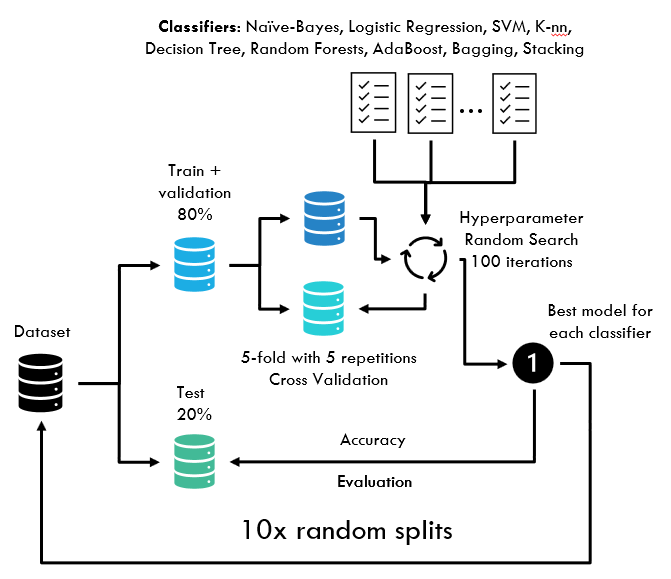
\includegraphics[width=0.5\textwidth]{soft_model_protocol.png}
      \caption{Soft Classifiers model validation protocol with hyperparameters search}
      \label{fig:soft_model_protocol}
\end{figure}

For each split, a model is selected as being the best parameter realization (of 100) in the 5x 5-fold cross validation and the best model (minimal validation loss) is then evaluated over the holdout set. By this procedure is possible to have the performance of the soft classifiers in ten different train/validation/test randomly generated splits.

A more complete reference on the soft classifiers algorithms tested in this work can be found in \cite{geron2017hands-on}


%    ____ _        _    ____ ____ ___ _____ ___ _____ ____  ____
%   / ___| |      / \  / ___/ ___|_ _|  ___|_ _| ____|  _ \/ ___|
%  | |   | |     / _ \ \___ \___ \| || |_   | ||  _| | |_) \___ \
%  | |___| |___ / ___ \ ___) |__) | ||  _|  | || |___|  _ < ___) |
%   \____|_____/_/__ \_\____/____/___|_|   |___|_____|_| \_\____/
%  |  _ \| ____/ ___|| | | | | |_   _|
%  | |_) |  _| \___ \| | | | |   | |
%  |  _ <| |___ ___) | |_| | |___| |
%  |_| \_\_____|____/ \___/|_____|_|

\subsection{Classifiers Results}

After training the neural network and performing a hyperparameter search for the soft models, the results over the 10 randomly generated tran/test splits is shown in \ref*{fig:results}. The average score is represented by the black dot.

\begin{figure}[H]
      \centering
      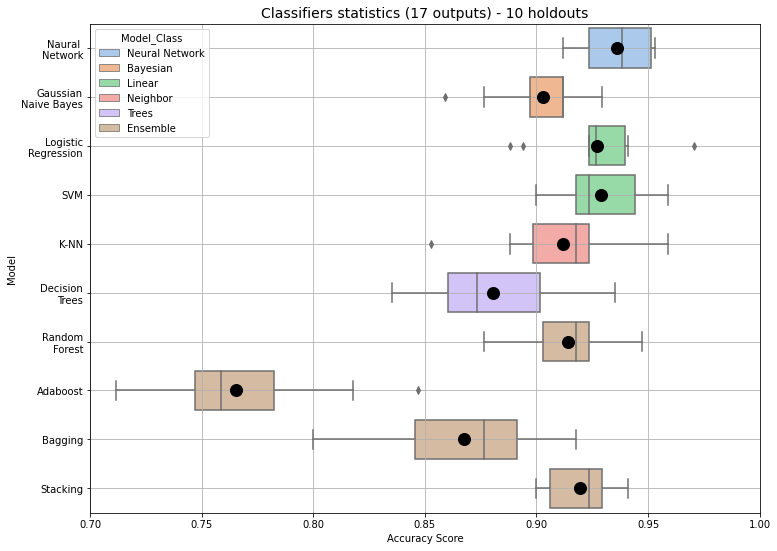
\includegraphics[width=0.5\textwidth]{results.png}
      \caption{Artificial Neural Network and soft classifiers results on predicting the 17 state conditions}
      \label{fig:results}
\end{figure}

The neural network classifier had the highest score over the classification task when compared to the other models, although the methodology implemented was not exactly the same. The linear models (Support Vector Machines and Multiclass Logistic Regression - Softmax) also had a quite high accuracy when compared to the others algorithms.

Decision Trees and the Ensemble methods showed a higher variance on their predictions and the best model of these was the Stack classifier using LogisticRegression, SVC, k-Neighbors classifier and RandomForest Classifier as estimators, but each of them with their default parameters.

%   _  __     _                              __  __
%  | |/ /___ | |__   ___  _ __   ___ _ __   |  \/  | __ _ _ __
%  | ' // _ \| '_ \ / _ \| '_ \ / _ \ '_ \  | |\/| |/ _` | '_ \
%  | . \ (_) | | | | (_) | | | |  __/ | | | | |  | | (_| | |_) |
%  |_|\_\___/|_| |_|\___/|_| |_|\___|_| |_| |_|  |_|\__,_| .__/

\section{Kohonen Map}

Kohonen or Self-Organizing Maps are a kind of neural network used to cluster the data into groups. Usually the neurons are organized in a 2-D so that the proximity in the input space is preserved in the 2D space after training. It's an unsupervised method that uses the technique of competitive learning and was proposed by \cite{kohonen}.

The final step of this study is to apply a self organizing map to the input data. The self organizing map trained was a 12x15 neurons. The darker values in the map shown in figure \ref*{fig:som_unsup} show neurons quite distant from their neighbors, what is interpreted as a separation between clusters. The map pattern shows two well separated regions, what is confirmed when we plot the labeled data in a binary level (damged x undamaged - figure \ref*{fig:som2}). The map is quite accurate in separating these two classes and detecting the presence of two groups of similar characteristics.

When we plot the labeled data with a more detail in classificatiom (4 groups or 17 state conditions), we see elements from the same class located in opposite positions in the map, what suggests that the map trained was not capable of separating groups in that level of detail (figures \ref*{fig:som4} and \ref*{fig:som17}).

Although we can see some coherence in figures \ref*{fig:som4} and \ref*{fig:som17} for some classes, the average quality of the map is poor.

\begin{figure*}
      \centering
      \begin{subfigure}{0.45\textwidth}
            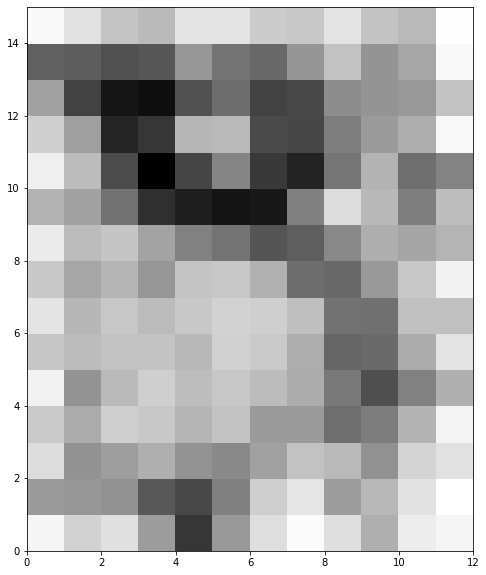
\includegraphics[width=\textwidth]{som_unsup.png}
            \caption{no label}
            \label{fig:som_unsup}
      \end{subfigure}
      \begin{subfigure}{0.45\textwidth}
            \centering
            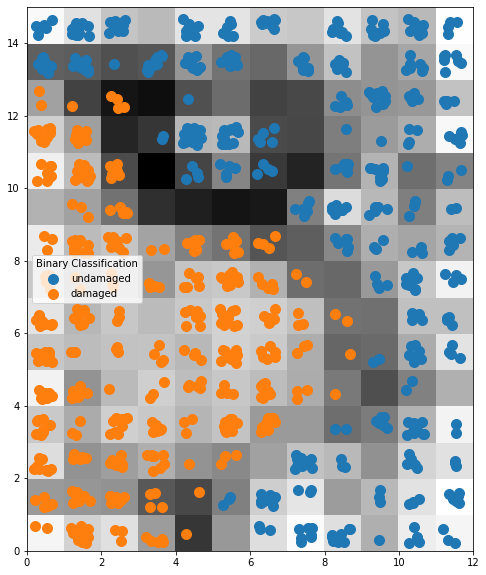
\includegraphics[width=\textwidth]{som_2.png}
            \caption{Binary classification: damage x undamaged}
            \label{fig:som2}
      \end{subfigure}
      \begin{subfigure}{0.45\textwidth}
            \centering
            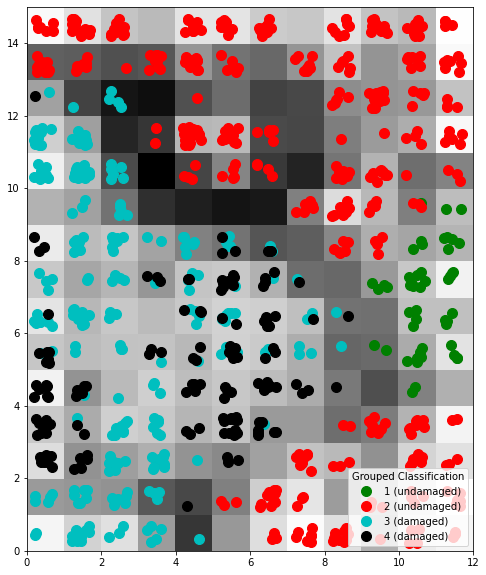
\includegraphics[width=\textwidth]{som_4.png}
            \caption{Grouped States}
            \label{fig:som4}
      \end{subfigure}
      \begin{subfigure}{0.45\textwidth}
            \centering
            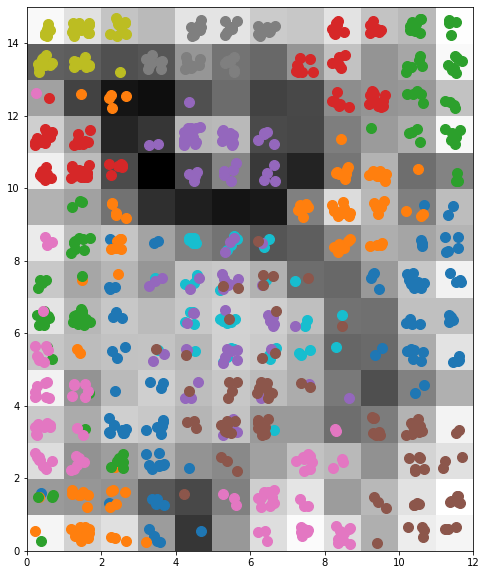
\includegraphics[width=\textwidth]{som_17.png}
            \caption{17 state conditions}
            \label{fig:som17}
      \end{subfigure}

      \caption{Self organizing map on background (a) and target labels plotted (b,c,d)}
      \label{fig:som}
\end{figure*}

%
%    ____ ___  _   _  ____ _    _   _ ____ ___ _   _  ____
%   / ___/ _ \| \ | |/ ___| |  | | | |  _ \_ _| \ | |/ ___|
%  | |  | | | |  \| | |   | |  | | | | | | | ||  \| | |  _
%  | |__| |_| | |\  | |___| |__| |_| | |_| | || |\  | |_| |
%   \____\___/|_|_\_|\____|_____\___/|____/___|_| \_|\____|
%  |  _ \| ____|  \/  |  / \  |  _ \| |/ / ___|
%  | |_) |  _| | |\/| | / _ \ | |_) | ' /\___ \
%  |  _ <| |___| |  | |/ ___ \|  _ <| . \ ___) |
%  |_| \_\_____|_|  |_/_/   \_\_| \_\_|\_\____/

\section{Concluding Remarks}

As the main conclusions of this study, we can mention:

\begin{enumerate}
      \item AR models, when using an appropriate order, are indeed useful as a feature extractor for the problem presented, and the coefficients of that model are themselves features in the reduced space.
      \item For the proposed problem, the PCA techinque was responsible for achieving a high comression in the feature space dimension, transforming a 120 dimension input space into a 6-component with only a few loss of information.
      \item The neural network model as well as the other classifiers (specially the linear models) performed well in detecting damage in the studied laboratory structure, considering the pre-processing procedures implemented (feature extraction and dimensionallity reduction).
      \item It's reasonable to think that the same neural network or any of the soft classifiers, if applied directly to the initial feature space would lead to a poor performance as classifiers, due to the huge amount of fetures, what shows the importance of the preliminary steps in a data processing pipeline.
      \item Self-Organizing Map trained in this study was capble of capturing the groups at a high level (binary classification: damaged vs undamaged), but showed a weak performance when getting in more detailed classification degrees.
\end{enumerate}

\bibliographystyle{apalike}
\bibliography{export}

\end{document}
